% Causal Restructuring: zero-shot results write-up.
% Overleaf: upload this file together with
%   restructuring_accuracy.png, restructuring_agreement.png, resnet18_selection_controls.png
% (all in results/) into the same project folder, then compile with pdfLaTeX.
\documentclass[11pt]{article}
\usepackage[margin=1in]{geometry}
\usepackage{amsmath,amssymb}
\usepackage{graphicx}
\usepackage{booktabs}
\usepackage{multirow}
\usepackage{caption}
\usepackage[hidelinks]{hyperref}
\usepackage{xcolor}

\newcommand{\best}[1]{\textbf{#1}}
\DeclareMathOperator*{\argmax}{arg\,max}
\DeclareMathOperator{\KL}{KL}

\title{Causal Restructuring of Neural Networks:\\Least-Squares Reconstruction and Sensitivity-Aware Budgets}
\author{Alexander Doyle}
\date{}

\begin{document}
\maketitle

\begin{abstract}
We study \emph{restructuring}, the removal of most of a trained network's units such that the remaining
network still reproduces the original's behaviour without retraining. Our pipeline ranks units by a
causal ablation score, selects a subset per layer, and repairs the weights downstream of the removed units.
We find that two changes to the original causal-restructuring framework account for nearly all of the gains.
The first is to replace the heuristic $1/\sqrt{|m|}$ weight folding with a closed-form least-squares
reconstruction of the next layer's input. The second is to allocate the unit budget across layers from
measured per-layer sensitivity curves. On UCI digits MLPs (5 seeds), the combined method retains
$93.4\%$ accuracy with $10\%$ of units kept, against $42.6\%$ for DeepAbstract; the teacher reaches
$98.2\%$. On ResNet-18/CIFAR-10 it reaches $42.9\%$, $59.2\%$ and $70.7\%$ zero-shot accuracy at $10\%$,
$20\%$ and $30\%$ of units kept, against $13.4\%$, $15.3\%$ and $28.6\%$ for DeepAbstract. Controls show
that the causal score is responsible for unit selection: under identical reconstruction it outperforms
k-means and random selection by large margins.
\end{abstract}

\section{Introduction}
Abstraction-based compression replaces groups of similar neurons by a single representative. It was
proposed as a way to make formal verification tractable~\cite{ashok2020deepabstract}. The quality of such
an abstraction depends on two choices. One is \emph{which} units survive. The other is \emph{how} the
weights are repaired to compensate for the removed ones. DeepAbstract selects representatives by k-means
on activation vectors and repairs weights by summing outgoing columns. Our framework instead selects units
by a causal intervention score, clusters the rest by cosine similarity of their activation fingerprints,
and repairs weights by averaging and folding.

This report evaluates the framework and three extensions to it in the zero-shot regime, with no
fine-tuning after restructuring. This isolates the quality of the restructuring itself.

\section{Method}
\label{sec:method}

\paragraph{Notation.}
Layer $\ell$ produces post-activation units $h_\ell(x)\in\mathbb{R}^{n_\ell}$. For convolutional layers a
unit is a channel. $W_{\ell+1}$ denotes the weights of the layer that consumes $h_\ell$, and $z(x)$ denotes
the logits. Restructuring keeps a set $K_\ell$ of units in each layer and masks the rest. The keep fraction
is $\kappa=\sum_\ell|K_\ell|/\sum_\ell n_\ell$.

\subsection{Causal scores and fingerprints}
For each unit $i$ we compute an \emph{activation fingerprint}
$\phi_i=(\bar h_i(x_1),\dots,\bar h_i(x_N))$ over $N$ calibration inputs, where $\bar h$ is the spatial
mean for channels. We also compute a \emph{causal ablation score}
\begin{equation}
  S_i = 1-\frac{1}{N}\sum_{n=1}^N \cos\!\big(z(x_n),\,z^{(i)}(x_n)\big),
\end{equation}
where $z^{(i)}$ denotes the logits with unit $i$ set to zero. $S_i$ measures the effect of removing the
unit, not the size of its activation.

\subsection{Selection}
In the original framework, the top $r\%$ of units by $S_i$ are reserved. The remaining (background) units
are clustered by average-linkage agglomerative clustering under the cosine distance
$d(i,j)=1-\cos(\phi_i,\phi_j)$. Each cluster contributes one medoid, chosen by
\begin{equation}
  m_C=\arg\min_{i\in C}\;(1-w)\big(1-\cos(\phi_i,\mu_C)\big)+w\Big(1-\tfrac{S_i}{\max_{j\in C}S_j}\Big),
\end{equation}
with $w=0.5$. Units that never activate on the calibration set are excluded from clustering, and they
are never chosen as medoids. We write $s$ for the \emph{reserve share}, the fraction of kept units that
come from the reserve. With $s=1$ the method reduces to keeping the top-$S_i$ units of each layer.

\subsection{Reconstruction}
\paragraph{Folding (original).} Each medoid's incoming weights, bias and BatchNorm affine parameters
become the cluster average. The removed members' outgoing columns are added to the medoid's column:
$W_{\ell+1}[:,m]\mathrel{+}=|C|^{-1/2}\sum_{j\in C\setminus m}W_{\ell+1}[:,j]$.

\paragraph{Least-squares reconstruction (LSQ).} We seek $W',b'$ minimising
$\mathbb{E}_x\lVert W h+b-(W'h_K+b')\rVert^2$. With layer mean $\mu$ and covariance $\Sigma$, this is the
linear regression of every unit onto the kept units:
\begin{equation}
  A=\Sigma_{:,K}\,(\Sigma_{KK}+\lambda I)^{-1},\qquad c=\mu-A\mu_K,\qquad
  W'=W A,\qquad b'=b+Wc,
\end{equation}
with ridge $\lambda=10^{-3}\operatorname{tr}(\Sigma_{KK})/|K|$. For convolutions, $\mu$ and $\Sigma$ are
pooled over samples and spatial positions, and $A$ is applied at every kernel offset. Kept units retain
their original incoming weights.

\paragraph{Residual streams.} In ResNets, the outputs of the last convolution of each block enter the skip
path and are consumed by several later layers. These units are masked but not folded.

\paragraph{BatchNorm.} After restructuring, the running statistics are re-estimated as a cumulative
average over 50 calibration batches.

\subsection{Sensitivity-aware budget}
For each layer $\ell$ and keep ratio $q\in\{0.05,0.1,0.2,\dots,1\}$, we restructure that layer alone
and record $D_\ell(q)=\mathbb{E}_x\,\KL\big(p_T(x)\,\|\,p_{\ell,q}(x)\big)$ on 512 calibration inputs.
After enforcing monotonicity, we solve
\begin{equation}
  \min_{\{q_\ell\}}\sum_\ell D_\ell(q_\ell)\quad\text{s.t.}\quad\sum_\ell n_\ell q_\ell=\kappa\sum_\ell n_\ell
\end{equation}
greedily, at each step lowering the keep ratio of the layer with the smallest increase in KL per unit
removed.

\subsection{Richer fingerprints}
As a third extension, fingerprints are computed on more samples and over a $2\times2$ spatial grid instead
of the global spatial mean.

\section{Experimental setup}
\paragraph{Models and data.} We use a 3-layer and a 5-layer MLP on UCI handwritten digits. Teachers are
trained with Adam (learning rate $10^{-3}$) for 30 epochs, and we report the mean over 5 teacher seeds.
We also use a CIFAR-style ResNet-18 on CIFAR-10, with one teacher reaching $90.1\%$ test accuracy.

\paragraph{Calibration.} Causal scores use 256 validation inputs. LSQ statistics use 2048 training inputs,
and sensitivity profiles use 512 training inputs.

\paragraph{Baseline.} The baseline is DeepAbstract~\cite{ashok2020deepabstract}, run at the same keep
fractions.

\paragraph{Metrics.} We report zero-shot test accuracy and \emph{agreement},
$\Pr[\argmax g(x)=\argmax f(x)]$, the fraction of test inputs on which the restructured network predicts
the teacher's class. As a consistency check, every reported pair satisfies
$\text{acc}-\text{agr}\le 100-\text{acc}_T$.

\section{Results}

\begin{figure}[t]
  \centering
  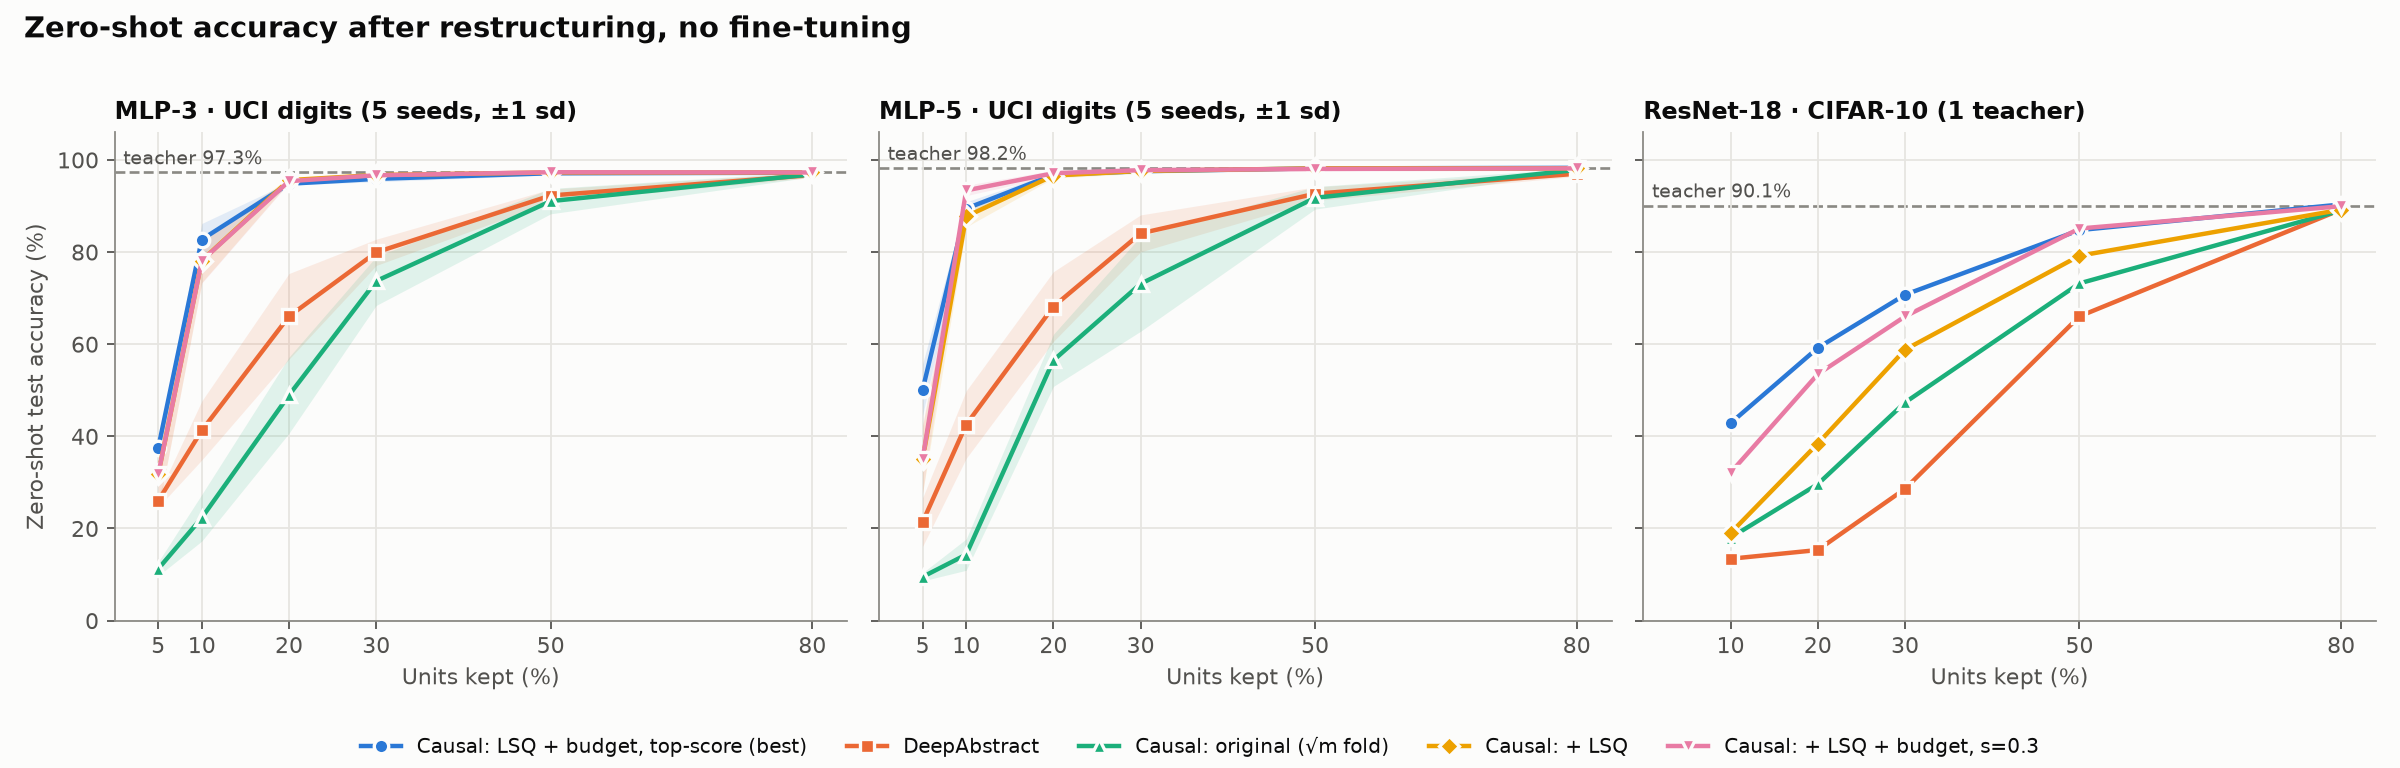
\includegraphics[width=\textwidth]{restructuring_accuracy.png}
  \caption{Zero-shot test accuracy against the percentage of units kept. The MLP panels show means over
  5 teacher seeds with $\pm1$ standard deviation bands. The dashed line is teacher accuracy.}
  \label{fig:acc}
\end{figure}

\begin{figure}[t]
  \centering
  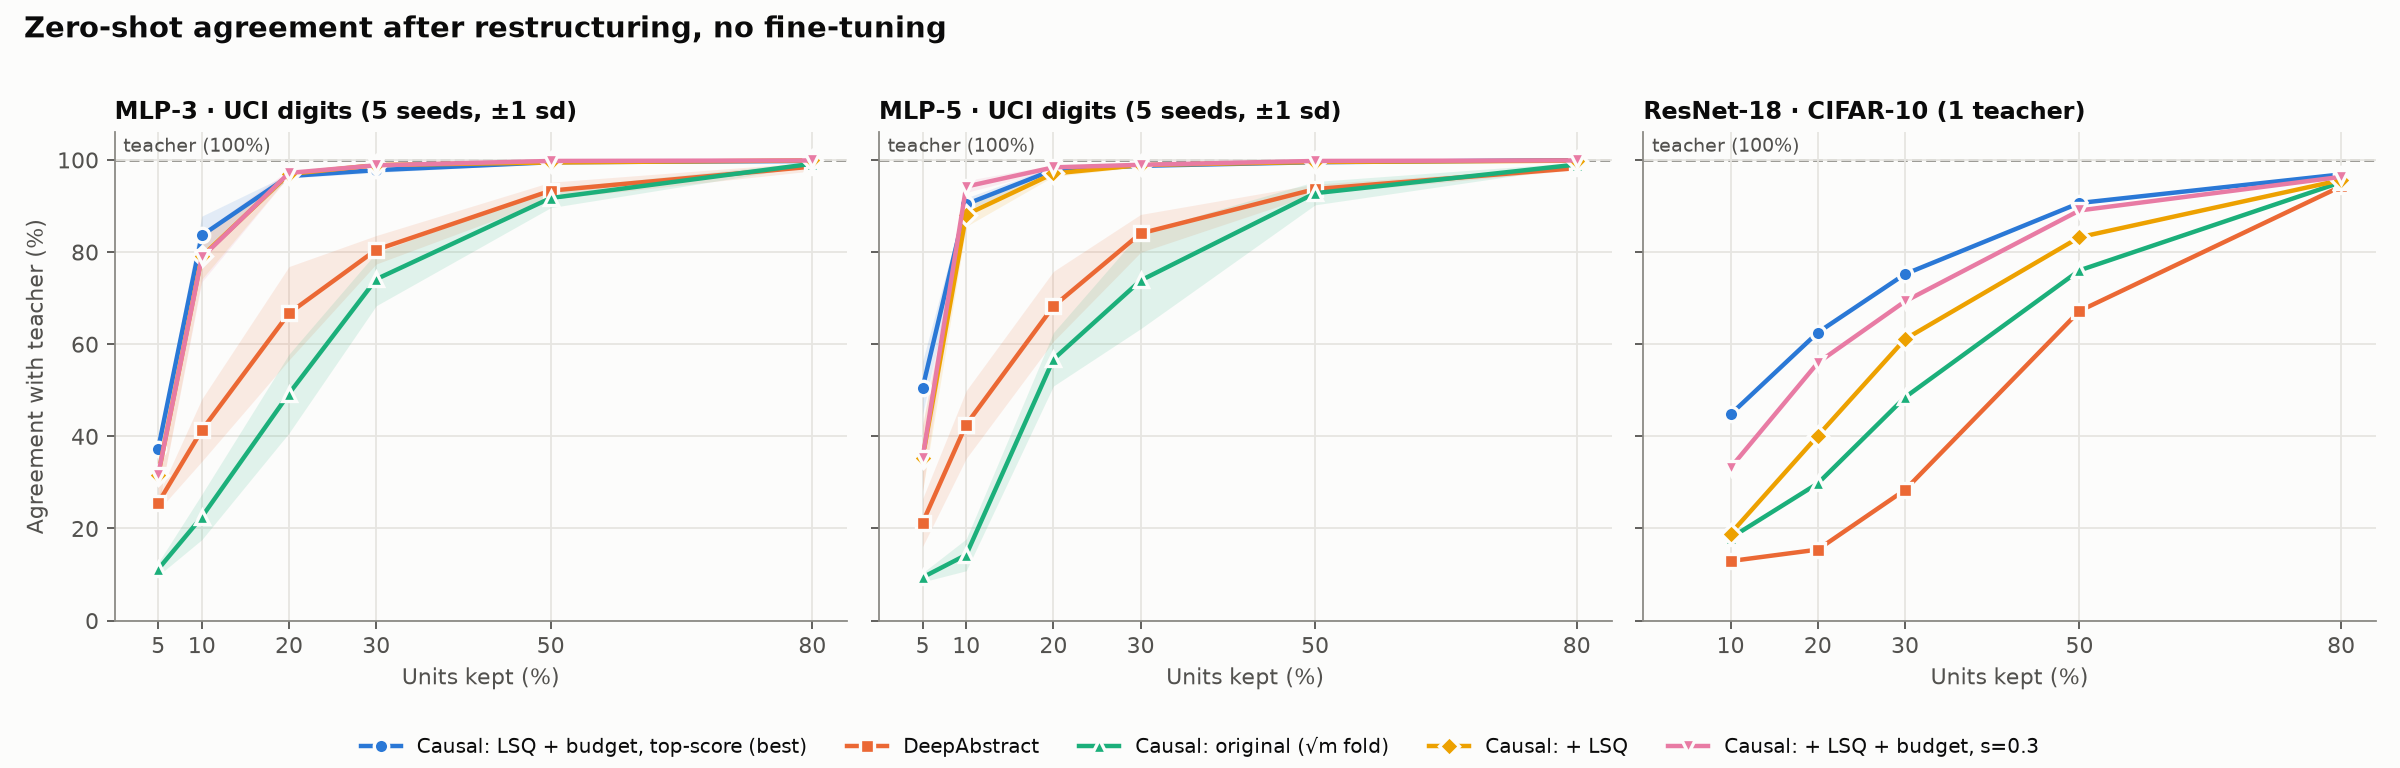
\includegraphics[width=\textwidth]{restructuring_agreement.png}
  \caption{Agreement with the teacher's predictions against the percentage of units kept.}
  \label{fig:agr}
\end{figure}

\paragraph{MLPs.} Table~\ref{tab:mlp} and Figure~\ref{fig:acc} show that LSQ is the dominant improvement.
On MLP-5 at $10\%$ kept, it lifts accuracy from $14.3\%$ to $87.7\%$, and adding the budget raises it
further to $93.4\%$. The budget alone, with folding, helps only moderately. Pure top-score selection
($s=1$) is best at $5\%$ kept. Mixing in clustered medoids ($s=0.3$) is marginally better between
$10\%$ and $30\%$ kept.

\begin{table}[t]
\centering
\caption{MLPs on UCI digits: zero-shot test accuracy (\%), mean over 5 seeds. Teacher accuracy is
$97.3\%$ (MLP-3) and $98.2\%$ (MLP-5). Columns give the percentage of units kept; bold marks the best
value in each column.}
\label{tab:mlp}
\small
\begin{tabular}{llcccccc}
\toprule
& Method & 5\% & 10\% & 20\% & 30\% & 50\% & 80\% \\
\midrule
\multirow{7}{*}{MLP-3}
& DeepAbstract                 & 26.0 & 41.3 & 66.1 & 79.9 & 92.3 & 96.7 \\
& Causal (fold)                & 11.2 & 22.3 & 48.9 & 73.7 & 91.1 & 96.9 \\
& \quad + budget               & 11.2 & 18.6 & 63.7 & 76.6 & 92.9 & 97.1 \\
& \quad + LSQ                  & 31.7 & 78.2 & \best{95.6} & \best{96.7} & \best{97.3} & \best{97.3} \\
& \quad + LSQ + budget ($s{=}0.3$) & 31.7 & 78.1 & 95.4 & \best{96.7} & \best{97.3} & \best{97.3} \\
& \quad + LSQ + budget ($s{=}1$)   & \best{37.4} & \best{82.7} & 94.8 & 95.9 & 97.1 & 97.2 \\
& Top-score + LSQ (uniform)    & \best{37.4} & \best{82.7} & 94.7 & 95.4 & 97.0 & \best{97.3} \\
\midrule
\multirow{7}{*}{MLP-5}
& DeepAbstract                 & 21.4 & 42.6 & 68.2 & 84.1 & 92.7 & 97.0 \\
& Causal (fold)                &  9.5 & 14.3 & 56.5 & 73.1 & 91.8 & 97.8 \\
& \quad + budget               &  9.5 & 18.5 & 60.0 & 79.4 & 94.2 & 98.2 \\
& \quad + LSQ                  & 35.0 & 87.7 & 96.6 & 97.6 & \best{98.2} & 98.2 \\
& \quad + LSQ + budget ($s{=}0.3$) & 35.0 & \best{93.4} & \best{97.1} & \best{97.8} & 98.1 & 98.2 \\
& \quad + LSQ + budget ($s{=}1$)   & \best{50.1} & 89.4 & 96.8 & 97.6 & \best{98.2} & \best{98.3} \\
& Top-score + LSQ (uniform)    & \best{50.1} & 87.7 & 96.1 & 97.4 & \best{98.2} & 98.2 \\
\bottomrule
\end{tabular}
\end{table}

\paragraph{ResNet-18.} Table~\ref{tab:resnet} shows that, unlike on the MLPs, the budget matters as much
as LSQ. Each helps alone, and the two are complementary. The best configuration is LSQ + budget with
$s=1$, which uses no clustering at all. At $10\%$ kept it reaches $42.9\%$ accuracy, against $13.4\%$ for
DeepAbstract and $18.0\%$ for the original framework. Its agreement with the teacher is the highest of all
methods at every keep fraction. Richer fingerprints do not change the results.

\begin{table}[t]
\centering
\caption{ResNet-18 on CIFAR-10 (teacher $90.1\%$): zero-shot accuracy / agreement (\%). Columns give the
percentage of units kept. Single teacher.}
\label{tab:resnet}
\small
\begin{tabular}{lccccc}
\toprule
Method & 10\% & 20\% & 30\% & 50\% & 80\% \\
\midrule
DeepAbstract                          & 13.4 / 12.9 & 15.3 / 15.4 & 28.6 / 28.4 & 66.0 / 67.2 & 89.2 / 94.3 \\
Causal (fold)                         & 18.0 / 17.9 & 29.6 / 29.8 & 47.3 / 48.5 & 73.2 / 76.0 & 89.0 / 95.2 \\
\quad + budget                        & 24.6 / 24.1 & 47.6 / 48.1 & 62.8 / 65.2 & 83.1 / 87.2 & 89.5 / 95.9 \\
\quad + LSQ                           & 19.0 / 18.9 & 38.4 / 40.1 & 58.8 / 61.1 & 79.2 / 83.2 & 89.2 / 95.6 \\
\quad + LSQ + budget ($s{=}0.3$)      & 32.1 / 33.2 & 53.5 / 56.0 & 66.0 / 69.3 & 85.1 / 89.0 & 90.0 / 96.3 \\
\quad + LSQ + budget ($s{=}0.5$)      & 32.5 / 33.2 & 54.0 / 56.1 & 69.3 / 72.7 & 84.8 / 89.5 & 90.1 / 96.7 \\
\quad + LSQ + budget ($s{=}0.5$) + $2{\times}2$ fp & 31.5 / 32.1 & 53.3 / 55.1 & 69.0 / 72.8 & \best{85.3} / 89.9 & 90.1 / 96.7 \\
\quad + LSQ + budget ($s{=}1$)        & \best{42.9} / \best{44.8} & \best{59.2} / \best{62.5} & \best{70.7} / \best{75.2} & 84.8 / \best{90.6} & \best{90.3} / \best{96.9} \\
\bottomrule
\end{tabular}
\end{table}

\paragraph{Which units to keep.} To separate selection from reconstruction, Figure~\ref{fig:controls}
applies the same LSQ reconstruction to four selection rules. Top-$S_i$ selection with a uniform
per-layer ratio outperforms k-means representatives (the DeepAbstract selection rule) at every keep
fraction, for example $51.7\%$ versus $33.3\%$ at $20\%$ kept. Random selection collapses to
$39.2\%$ even at $50\%$ kept. The sensitivity budget then adds most at the lowest keep fraction:
$42.9\%$ versus $19.9\%$ at $10\%$ kept.

\begin{figure}[t]
  \centering
  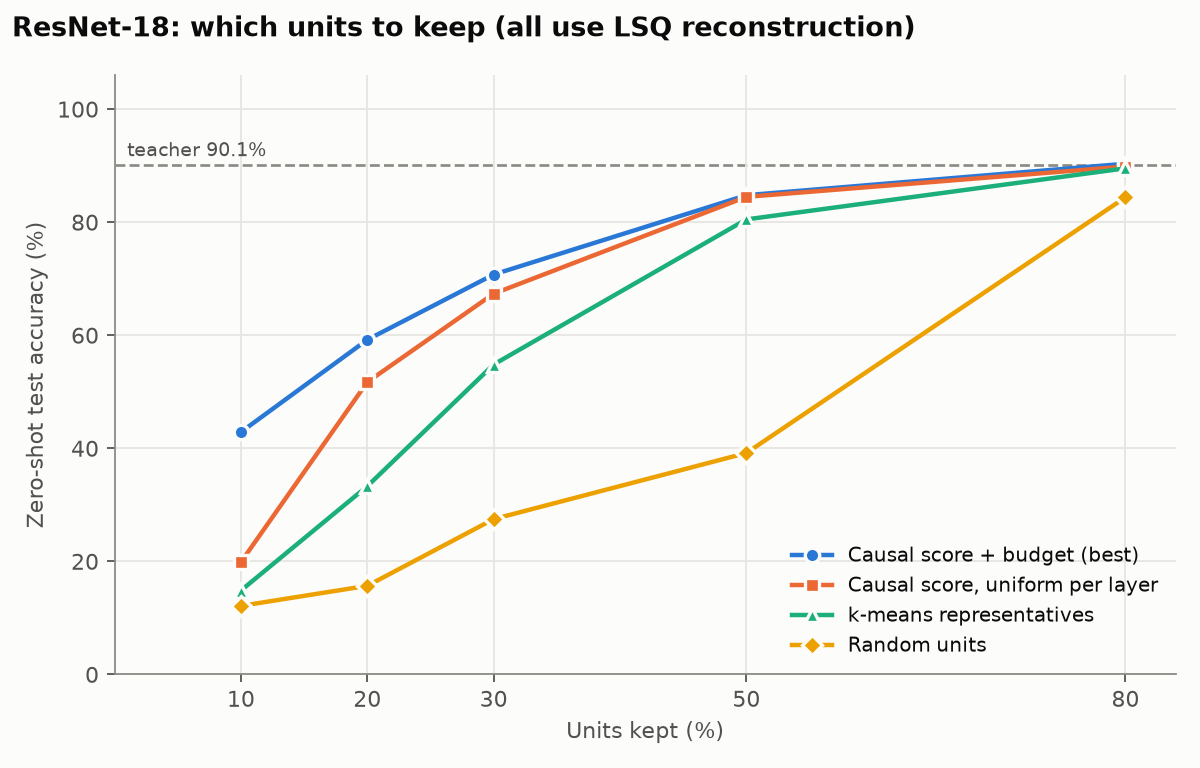
\includegraphics[width=0.7\textwidth]{resnet18_selection_controls.png}
  \caption{ResNet-18 selection controls. All four rules use LSQ reconstruction; only the choice of kept
  units differs.}
  \label{fig:controls}
\end{figure}

\section{Discussion}
The results separate the pipeline into three roles. The causal score ranks units \emph{within} a layer.
The sensitivity budget decides \emph{how many} units each layer keeps. LSQ \emph{repairs} what was
removed. Clustering, which in the original framework was meant to guarantee diversity among kept units,
becomes unnecessary on ResNet-18. One explanation is that units duplicated by a kept unit receive low
causal scores, because the duplicate compensates for their ablation. Any remaining redundancy is then
resolved by LSQ, which reconstructs every dropped unit from all survivors rather than from a single
medoid. The $1/\sqrt{|m|}$ fold, in contrast, is a fixed interpolation between the identical-unit and
uncorrelated-unit cases. It is optimal for neither, and averaging the medoid's incoming weights further
perturbs the unit that is kept.

\section{Limitations}
\begin{itemize}
  \item ResNet-18 results use a single teacher, so they carry no confidence intervals.
  \item The DeepAbstract baseline uses the original BatchNorm recalibration (momentum $0.1$), whereas our
        method uses a cumulative re-estimate. This may understate the baseline on ResNet-18.
  \item All results are zero-shot. The effect of knowledge-distillation fine-tuning on the gaps between
        methods is not measured here.
  \item ResNet-50 and larger datasets are not yet evaluated.
\end{itemize}

\begin{thebibliography}{9}
\bibitem{ashok2020deepabstract}
P.~Ashok, V.~Hashemi, J.~K\v{r}et\'{i}nsk\'{y}, and S.~Mohr.
\newblock DeepAbstract: Neural network abstraction for accelerating verification.
\newblock In \emph{Automated Technology for Verification and Analysis (ATVA)}, 2020.
\end{thebibliography}

\end{document}
